\documentclass{article}

\usepackage{tikz}

\begin{document}
\begin{figure}[h!]
  \begin{center}
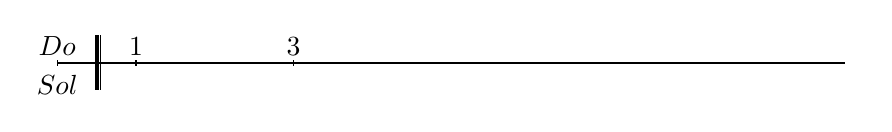
\begin{tikzpicture}
\draw[thick] (0,0) -- (10,0) node[anchor=north west] {}; % main ligne
\draw (0cm, 1pt) -- (0cm, -1pt) node [anchor=south] {$Do$};  % init ligne Do
\draw (0cm, 1pt) -- (0cm, -1pt) node [anchor=north] {$Sol$};  % init ligne Sol
\draw [line width=0.5mm ] (0.5cm, 10pt) -- (0.5cm, -10pt) node {}; % thick vertical ligne
\draw (0.55cm, 10pt) -- (0.55cm, -10pt) node {}; % second start vertical ligne
\foreach \x in { 1,3}
\draw(\x cm, 1pt)--(\x cm, -1pt) node[anchor = south] {$\x$};
\end{tikzpicture}
  \end{center}
\end{figure}
\end{document}
